%%%%%%%%%%%%%%%%%%%%%%%%%%%%%%%%%%%%%%%%%
% Beamer Presentation
% LaTeX Template
% Version 1.0 (10/11/12)
%
% This template has been downloaded from:
% http://www.LaTeXTemplates.com
%
% License:
% CC BY-NC-SA 3.0 (http://creativecommons.org/licenses/by-nc-sa/3.0/)
%
%%%%%%%%%%%%%%%%%%%%%%%%%%%%%%%%%%%%%%%%%

%----------------------------------------------------------------------------------------
%	PACKAGES AND THEMES
%----------------------------------------------------------------------------------------

\documentclass[aspectratio=169, 9pt]{beamer}

\mode<presentation> {

% The Beamer class comes with a number of default slide themes
% which change the colors and layouts of slides. Below this is a list
% of all the themes, uncomment each in turn to see what they look like.

%\usetheme{default}
%\usetheme{AnnArbor}
%\usetheme{Antibes}
%\usetheme{Bergen}
%\usetheme{Berkeley}
%\usetheme{Berlin}
%\usetheme{Boadilla}
%\usetheme{CambridgeUS}
%\usetheme{Copenhagen}
%\usetheme{Darmstadt}
%\usetheme{Dresden}
%\usetheme{Frankfurt}
%\usetheme{Goettingen}
%\usetheme{Hannover}
%\usetheme{Ilmenau}
%\usetheme{JuanLesPins}
%\usetheme{Luebeck}
%\usetheme{Madrid}
\usetheme{Malmoe}
%\usetheme{Marburg}
%\usetheme{Montpellier}
%\usetheme{PaloAlto}
%\usetheme{Pittsburgh}
%\usetheme{Rochester}
%\usetheme{Singapore}
%\usetheme{Szeged}
%\usetheme{Warsaw}

% As well as themes, the Beamer class has a number of color themes
% for any slide theme. Uncomment each of these in turn to see how it
% changes the colors of your current slide theme.

%\usecolortheme{albatross}
%\usecolortheme{beaver}
%\usecolortheme{beetle}
%\usecolortheme{crane}
%\usecolortheme{dolphin}
%\usecolortheme{dove}
%\usecolortheme{fly}
%\usecolortheme{lily}
%\usecolortheme{orchid}
%\usecolortheme{rose}
%\usecolortheme{seagull}
%\usecolortheme{seahorse}
%\usecolortheme{whale}
%\usecolortheme{wolverine}

%\setbeamertemplate{footline} % To remove the footer line in all slides uncomment this line
%\setbeamertemplate{footline}[page number] % To replace the footer line in all slides with a simple slide count uncomment this line

%\setbeamertemplate{navigation symbols}{} % To remove the navigation symbols from the bottom of all slides uncomment this line
}

\usepackage{xcolor}

\definecolor{han_purple}{rgb}{0, 0.28, 0.80}
\definecolor{beige}{rgb}{0.96, 0.92, 0.89}
\definecolor{lightgray}{rgb}{0.8, 0.8, 0.8}
\definecolor{blue}{HTML}{3066be}
\definecolor{green}{HTML}{43894e}
\definecolor{definition}{HTML}{0ABD1C}
\definecolor{theorem}{HTML}{0072A3}
\definecolor{proposition}{HTML}{FF4B3E}
\definecolor{orange}{HTML}{F5B400}
\definecolor{purple}{HTML}{30CC71}
\definecolor{red}{HTML}{eb9486}
\definecolor{lightgreen}{HTML}{72d5a3}
\definecolor{darkgreen}{HTML}{216e47}


\newcommand{\X}{\boldsymbol{X}}
\newcommand{\V}{\boldsymbol{V}}
\newcommand{\W}{\boldsymbol{W}}
\newcommand{\Y}{\boldsymbol{Y}}
\newcommand{\Q}{\boldsymbol{Q}}
\newcommand{\Z}{\boldsymbol{Z}}
\newcommand{\M}{\boldsymbol{M}}
\newcommand{\A}{\boldsymbol{A}}
\renewcommand{\H}{\boldsymbol{H}}
\newcommand{\B}{\boldsymbol{B}}
\newcommand{\D}{\boldsymbol{D}}
\newcommand{\R}{\boldsymbol{R}}
\renewcommand{\P}{\boldsymbol{P}}
\newcommand{\I}{\boldsymbol{I}}
\renewcommand{\L}{\boldsymbol{\Lambda}}
\renewcommand{\S}{\boldsymbol{\Sigma}}

\DeclareMathOperator*{\argmax}{arg\,max}
\DeclareMathOperator*{\argmin}{arg\,min}

\definecolor{physics}{HTML}{8EA604}
\definecolor{intrinsic}{HTML}{ec9f05}
\definecolor{semantic}{HTML}{818AA3}

%\definecolor{azure}{HTML}{728797}
\definecolor{coral}{HTML}{566876}
\definecolor{pin}{HTML}{005556}
\definecolor{pousse}{HTML}{00b57b}
\definecolor{ardoise}{HTML}{5b6770}

\usepackage{comment}
\usepackage{subcaption}
\usepackage{bibentry}
\usepackage{amsmath}
\usepackage{tabularray}[=v2021]
\usepackage{hyperref}

%\DeclareMathOperator*{\max}{arg\,min}
%\DeclareMathOperator*{\min}{arg\,max}

\usepackage{multirow}
\usepackage{enumitem}
\usepackage{subcaption}
\usepackage{makecell}
\usefonttheme[onlymath]{serif}
\usepackage{booktabs}
\usepackage{mathabx}
\usepackage{amssymb}

\usepackage{animate}

\newcommand{\x}{\boldsymbol{x}}
\newcommand{\z}{\boldsymbol{z}}
\newcommand{\param}{\boldsymbol{\theta}}
\newcommand{\phiparam}{\boldsymbol{\phi}}
\newcommand{\qphi}{q_{\phiparam}}
\newcommand{\zi}{\textcolor{red}{\z_I}}
\newcommand{\ze}{\textcolor{blue}{\z_E}}
\newcommand{\xk}[1]{\boldsymbol{x}^{(#1)}}
\newcommand{\yk}[1]{y^{(#1)}}
\newcommand{\vv}{\boldsymbol{v}}
\newcommand{\ppdf}{p_{\boldsymbol{\theta}}}
\newcommand{\fphi}{f_{\boldsymbol{\phi}}}

\renewcommand{\L}{\textcolor{blue}{L}}
\newcommand{\PW}{\textcolor{red}{PW}}


\newtheorem{thm}{Théorème}

\setbeamertemplate{page number in head/foot}[appendixframenumber] % stop page numebering after conclusion

\setbeamercolor{section in head/foot}{bg=coral!50!black, fg=white}
\setbeamercolor{frametitle}{fg=ardoise}
\setbeamercolor{structure}{fg=pin}
\setbeamercolor{title}{fg=ardoise}

\hypersetup{
    colorlinks,
    linkcolor={ardoise},
    citecolor={blue!80!black},
    urlcolor={ardoise}
}

%\hypersetup{colorlinks,urlbordercolor={1 1 1},linkcolor=,urlcolor=poussin}

%\setbeamercolor{footline}{bg=pin, fg=pin}

\newenvironment{madridblock}[1]
{
  \begin{block}{#1}
}
{
  \end{block}
}

\titlegraphic{
    
\includegraphics[height=0.8cm]{figures/logo_mia.png} \hspace{0cm}
    
\includegraphics[height=0.6cm]{figures/APT_Logo_RVB_Positif.png} \hspace{0cm}
    
\includegraphics[height=0.8cm]{figures/Logotype UPSaclay_RVB.png}
}

%\setbeamercolor{block title}{bg=coral!40,fg=black}
%\setbeamercolor{block body}{bg=coral!5,fg=black}

%\hypersetup{
%    colorlinks,
%    citecolor=han_purple,
%    linkcolor=han_purple
%}

%\newcommand{\vv}[1]{\textcolor{han_purple}{#1}}
%
%\DeclareFontFamily{U}{matha}{\hyphenchar\font45}
%\DeclareFontShape{U}{matha}{m}{n}{
%      <5> <6> <7> <8> <9> <10> gen * matha
%      <10.95> matha10 <12> <14.4> <17.28> <20.74> <24.88> matha12
%      }{}
%\DeclareSymbolFont{matha}{U}{matha}{m}{n}

\setbeamercovered{transparent}

\setbeamertemplate{headline}{}

\makeatletter
\def\normalcolor{\let\current@color\default@color\set@color\transparent{1}}
\makeatother
%----------------------------------------------------------------------------------------
%	TITLE PAGE
%----------------------------------------------------------------------------------------
\title{Anomaly detection for the monitoring of tree dieback \\ from multispectral satellite images}
\subtitle{The case of dark beetle infestations}

\author[Romain Thoreau]{
	Romain Thoreau \\ AgroParisTech - MIA Paris Saclay
	\\ \url{romain.thoreau@agroparistech.fr}
}

\institute[AgroParisTech]

\date{November 2026}


%\setbeamertemplate{footline}{}
\setbeamertemplate{navigation symbols}{}

\setbeamertemplate{footline}
{
  \leavevmode%
  \hbox{%
  \begin{beamercolorbox}[wd=.333333\paperwidth,ht=2.25ex,dp=1ex,center]{author in head/foot}%
    \usebeamerfont{author in head/foot}\insertshortauthor
  \end{beamercolorbox}%
  \begin{beamercolorbox}[wd=.333333\paperwidth,ht=2.25ex,dp=1ex,center]{title in head/foot}%
    \usebeamerfont{title in head/foot}\insertshortinstitute
  \end{beamercolorbox}%
  \begin{beamercolorbox}[wd=.333333\paperwidth,ht=2.25ex,dp=1ex,right]{date in head/foot}%
    \usebeamerfont{date in head/foot}\insertshortdate{}\hspace*{2em}
    \insertframenumber{} / \inserttotalframenumber\hspace*{2ex} 
  \end{beamercolorbox}}%
  \vskip0pt%
}


\setbeamercolor{textcitation}{fg=black,bg=beige}
\setbeamerfont{block body textcitation}{size=\tiny}

\begin{document}
%--------------------------------------------------------------------------
\begin{frame}
\titlepage % Print the title page as the first slide
\end{frame}
%%%-------------------------------------------------------------------------
\begin{frame}{Outline}
\tableofcontents
\end{frame}
%---------------------------------------------------------------------------

\begin{frame}{Bibliography and references}

\begin{itemize}[label=$\bullet$]
	\item This lecture is largely based on the presentation "Détection des problèmes sanitaires des forêts par imagerie satellite optique: principes et application au cas des scolytes de l’épicéa" by JB Féret, R Dutrieux, K Ose \& F de Boissieu in October 4, 2022 at Atelier Theia (\url{https://www.theia-land.fr/foret/2022-sante-foret/}) and associated publication (\url{https://www.onf.fr/onf/+/cec::les-rendez-vous-techniques-de-lonf-no69-70.html}).
\end{itemize}


\end{frame}
%--------------------------------------------------------------------------
\begin{frame}{Bark beetle infestation}

\begin{columns}

\column{0.15\textwidth}

\begin{figure}
	\center
	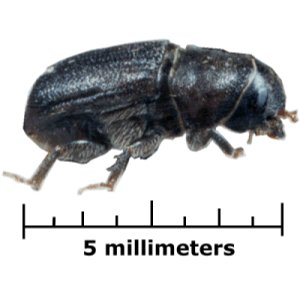
\includegraphics[width=\textwidth]{figures/Dendroctonus_ponderosae.jpeg}
	\caption{Bark Beetle. Source: Wikipedia}
\end{figure}


\column{0.4\textwidth}

\begin{figure}
	\center
	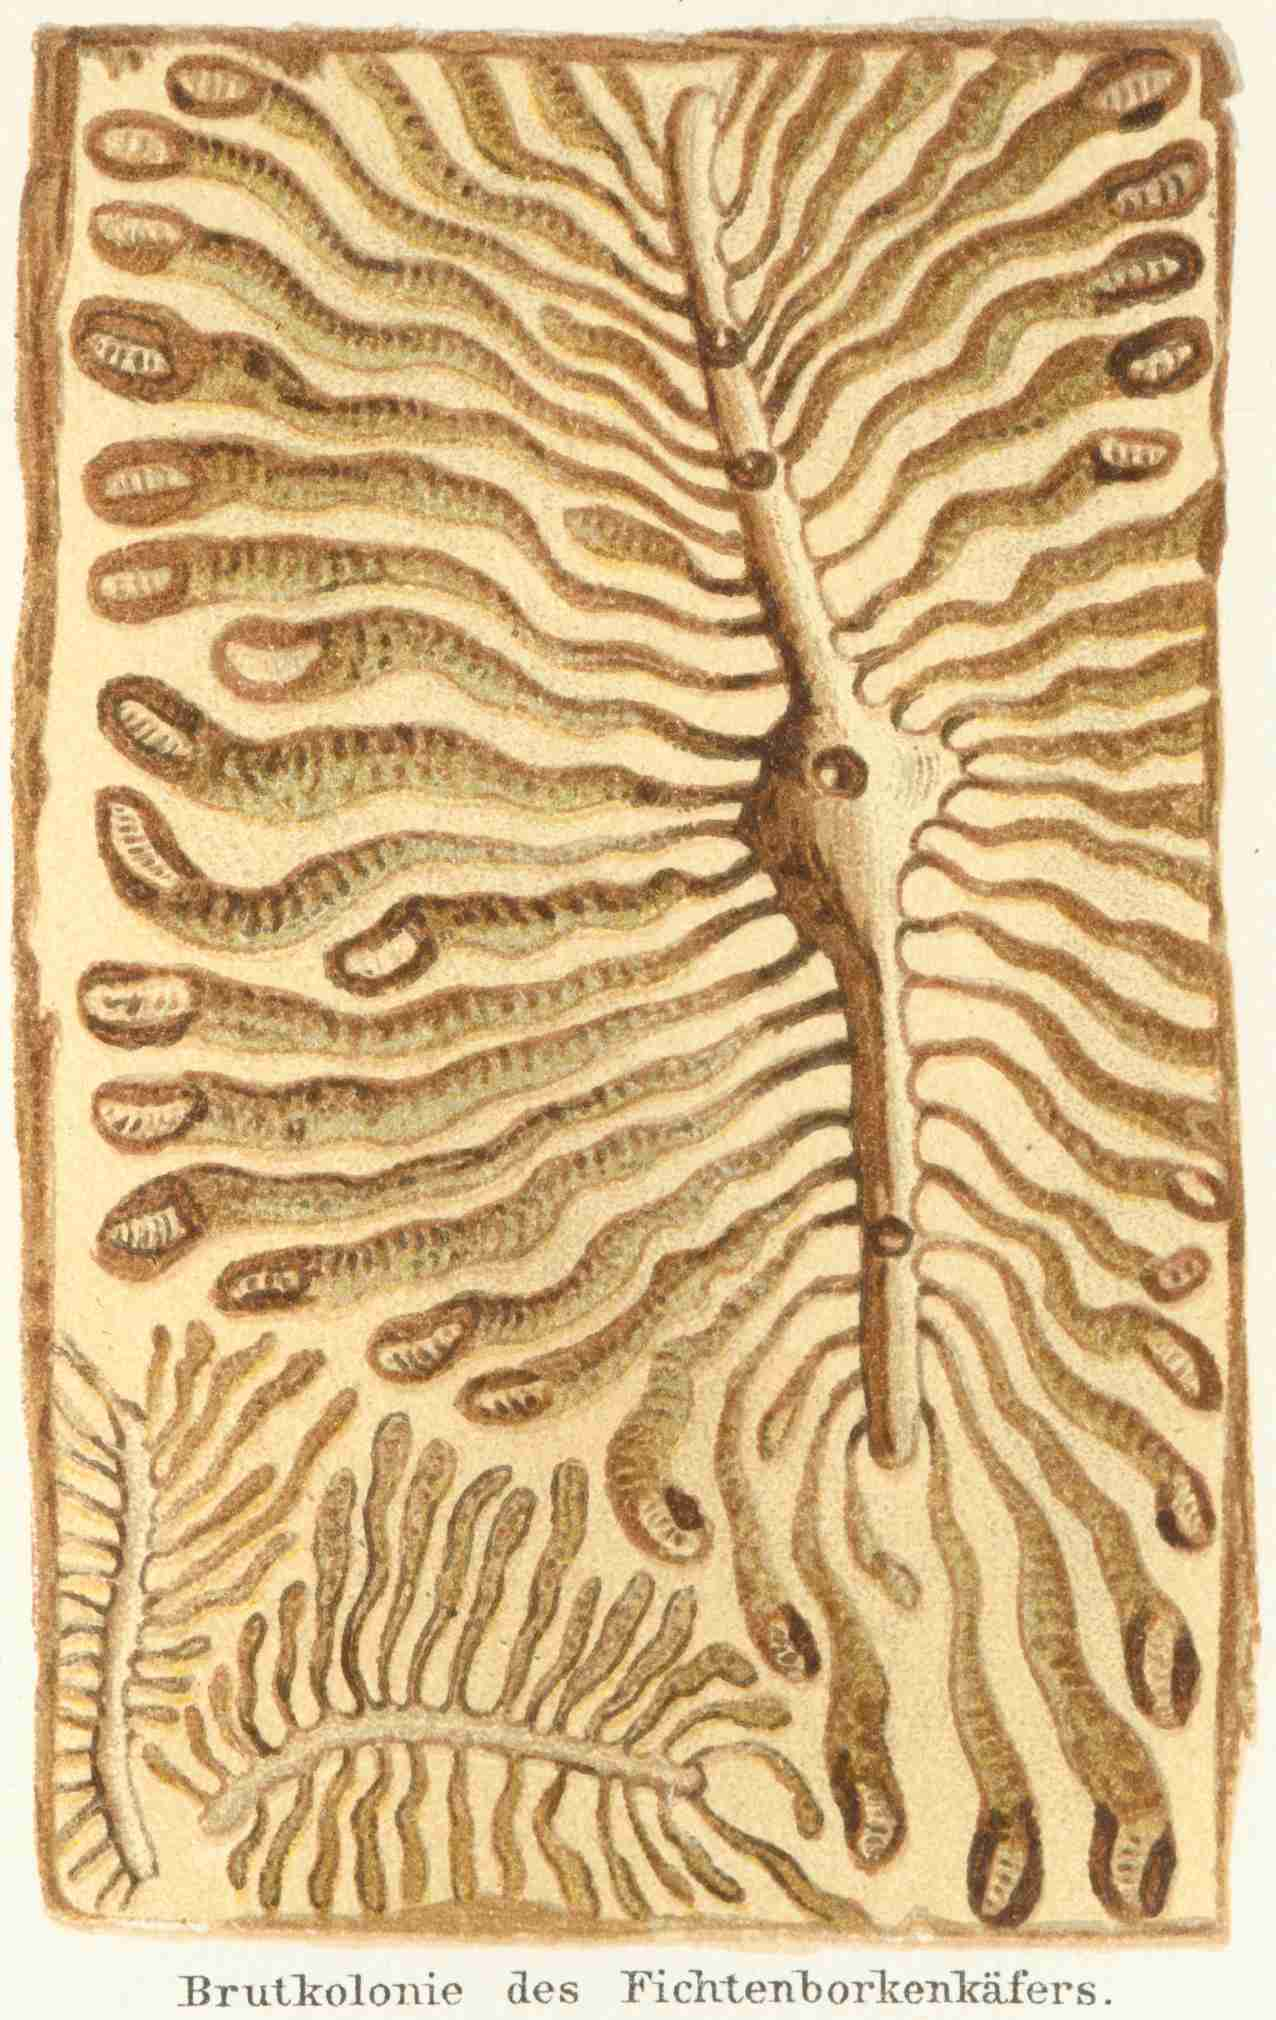
\includegraphics[width=0.5\textwidth]{figures/Ips_typographicus_2_meyers_1888_v16_p352.jpeg}
	\caption{The architecture of the tunnel system varies by species. In the typograph moth, the egg-laying tunnels are generally vertical, while the larval tunnels are horizontal and winding. Source: Wikipedia\footnotemark[1]}
\end{figure}

\column{0.3\textwidth}

\begin{figure}
	\center
	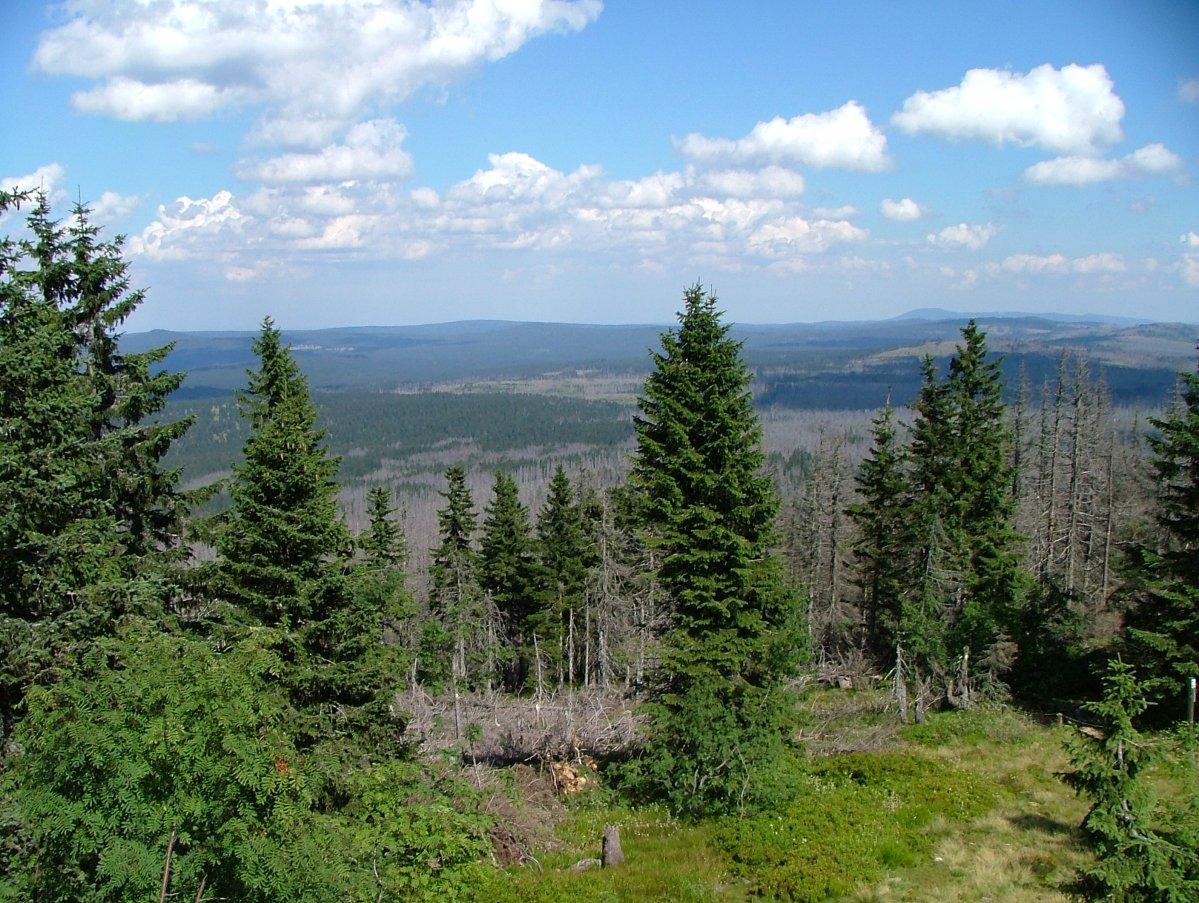
\includegraphics[width=\textwidth]{figures/Bayerischer_wald1.jpeg}
	\caption{Effects of bark beetle in the Bavarian Forest. Source: Wikipedia}
\end{figure}

\end{columns}


\footnotetext[1]{Meyers Konversations-Lexikon, 4. Aufl. 1888, Bd. 16, S. 352, Ausschnitt aus Tafel Waldverderber I (Käfer); Bd. 16, S. 352 aus Konversations-Lexikon im www[lien cassé], Domaine public, https://commons.wikimedia.org/w/index.php?curid=275883}

\end{frame}
%--------------------------------------------------------------------------
\begin{frame}{Monitoring of bark beetle infestation from multispectral satellite images}

\begin{figure}
	\center
	\begin{subfigure}{0.3\textwidth}
		\center
		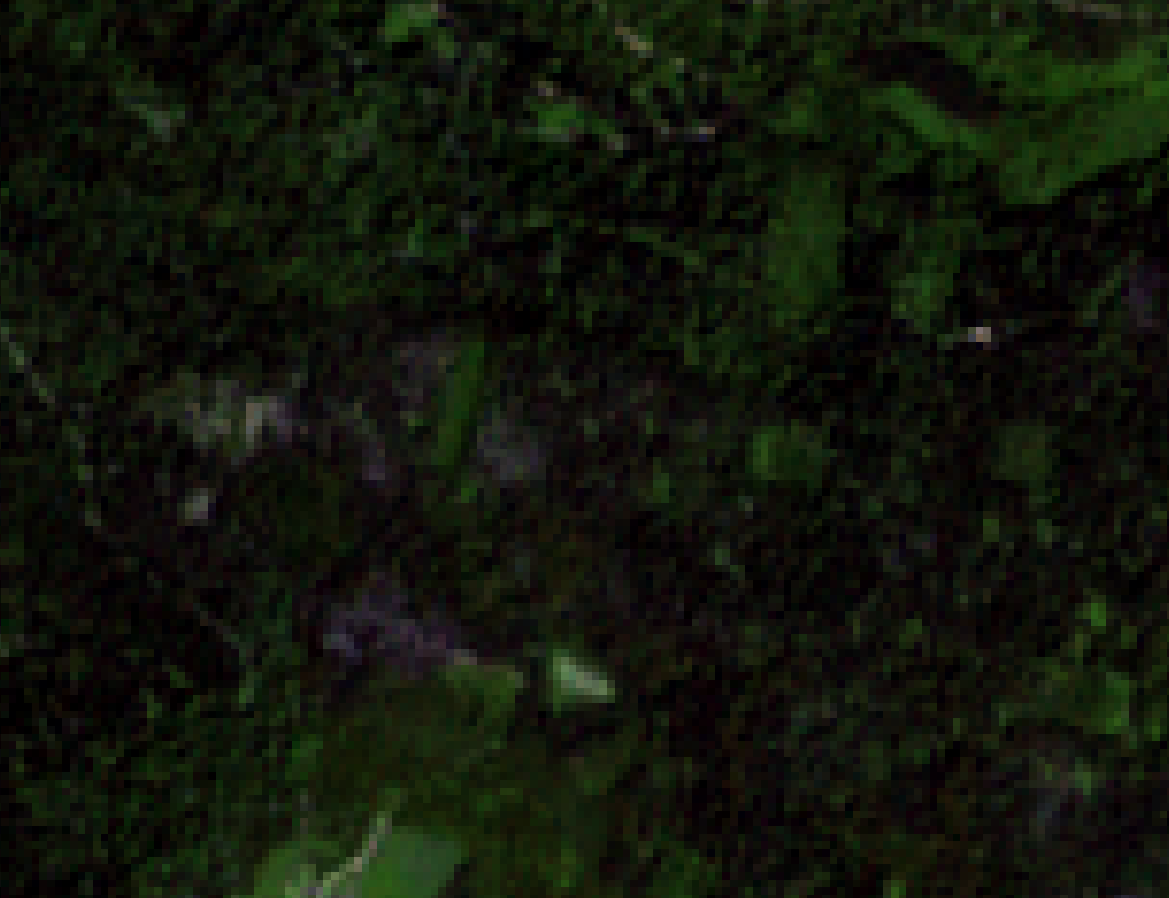
\includegraphics[width=\textwidth]{figures/ajol_2018.png}
		\caption{2018}
	\end{subfigure}
	\begin{subfigure}{0.3\textwidth}
		\center
		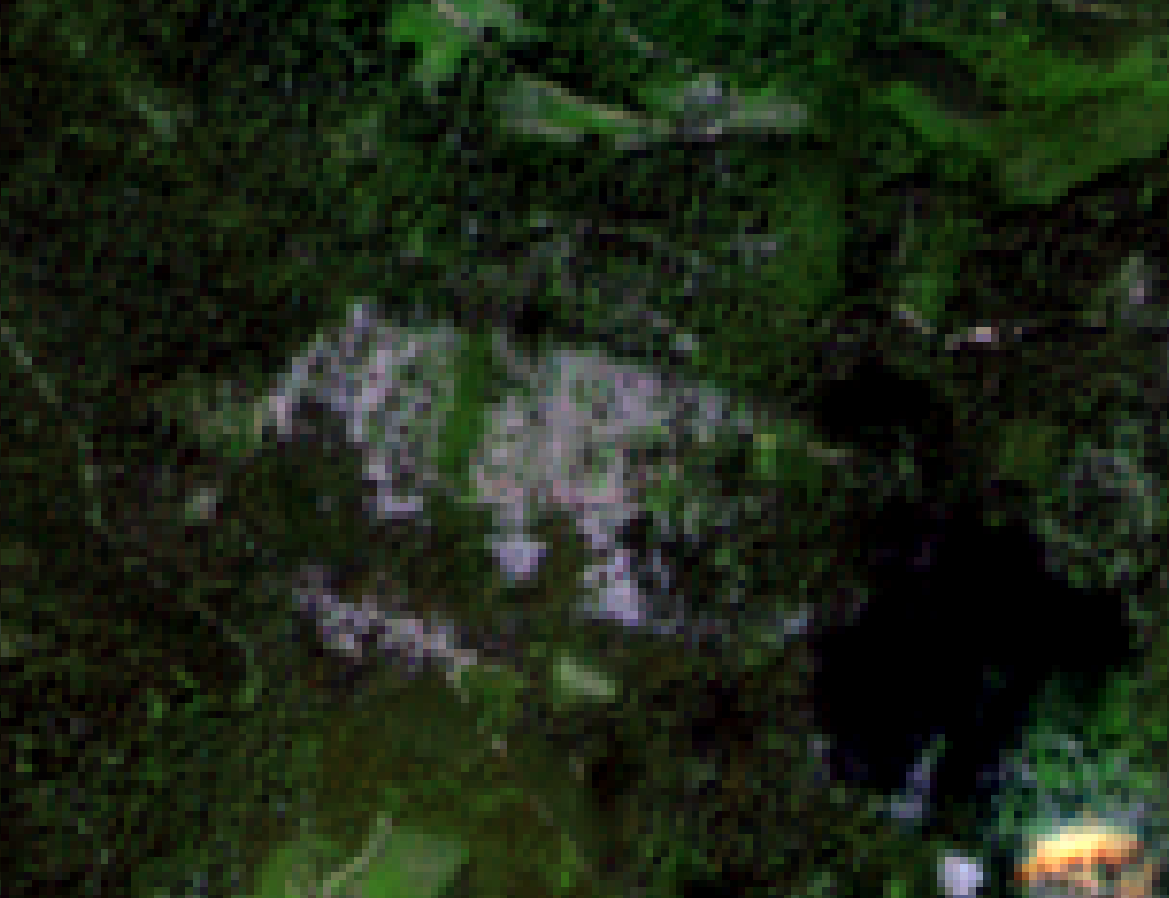
\includegraphics[width=\textwidth]{figures/ajol_2019.png}
		\caption{2019}
	\end{subfigure}
	\begin{subfigure}{0.3\textwidth}
		\center
		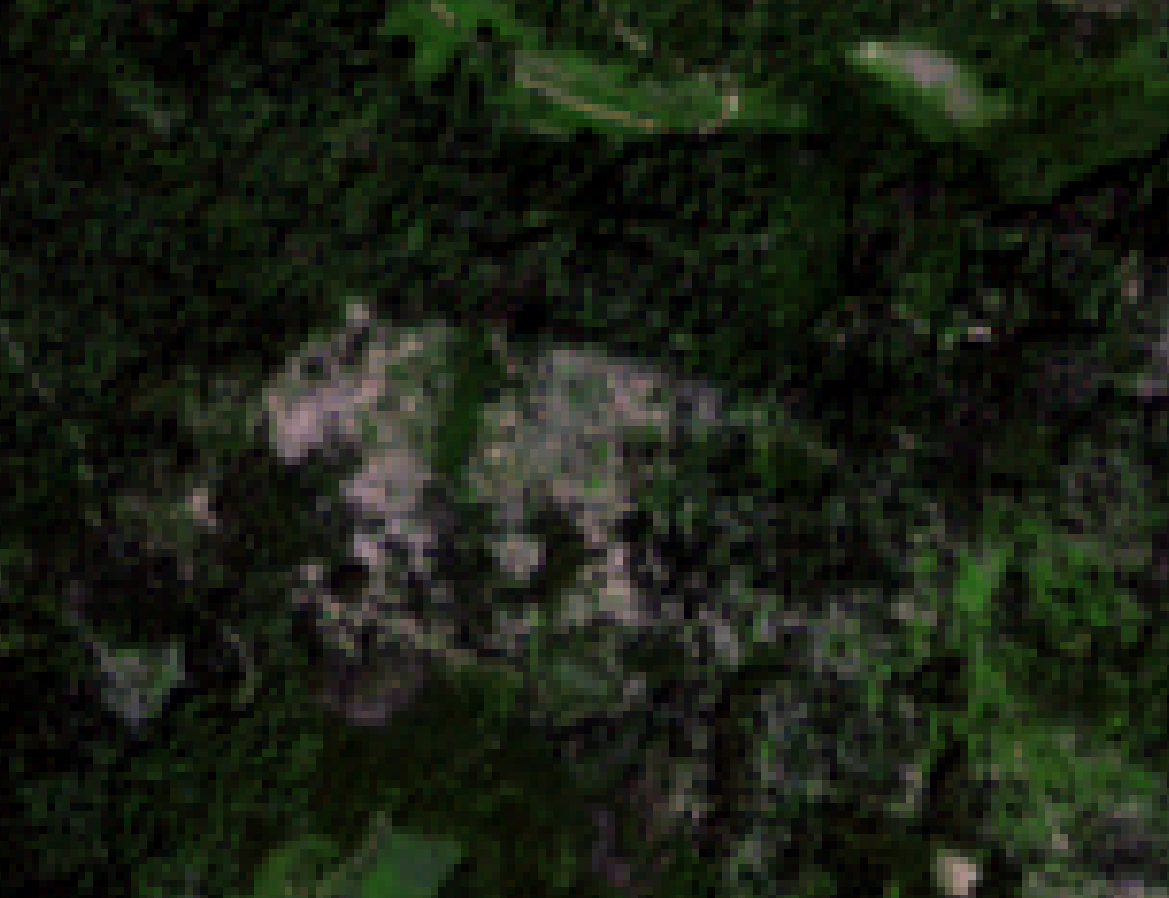
\includegraphics[width=\textwidth]{figures/ajol_2020.png}
		\caption{2020}
	\end{subfigure}
	\caption{RGB composition of Sentinel-2 images (ESA, Copernicus) - Val d'Ajol, France}
\end{figure}

\end{frame}
%--------------------------------------------------------------------------
\begin{frame}
	Let's start coding!
\end{frame}
%--------------------------------------------------------------------------
%\begin{frame}[allowframebreaks,noframenumbering]
%\frametitle{}
%	\scriptsize{
%	\bibliographystyle{apalike}
%	\bibliography{main}}
%\end{frame}

\end{document}
